\documentclass[12pt, a4paper]{ctexart}
\usepackage{geometry}
\geometry{left=2.5cm, right=2.5cm, top=3cm, bottom=3cm}
\usepackage{listings}
\usepackage{graphicx}
\usepackage{xcolor}
\usepackage{amsmath}
\usepackage{booktabs}
\usepackage{tikz}
\usetikzlibrary{positioning, arrows.meta}
\usepackage{float}

% Code snippet settings
\lstset{
    basicstyle=\ttfamily\small,
    frame=single,
    framesep=5pt,
    xleftmargin=10pt,
    xrightmargin=10pt,
    keywordstyle=\color{blue},
    commentstyle=\color{gray},
    breaklines=true
}

\begin{document}

% 封面
\begin{titlepage}
    \centering
    \vspace*{5cm}
    {\Huge\bfseries 实验报告\par}
    \vspace{2cm}
    {\Large 课程：数字逻辑与计算机组成实验\par}
    \vspace{1cm}
    {\Large 实验六：状态机及键盘输入\par}
    \vspace{4cm}
    {\large 姓名：\underline{\makebox[4cm]{郑袭明}}\par}
    \vspace{1cm}
    {\large 学号：\underline{\makebox[4cm]{251502027}}\par}
    \vspace{1cm}
    {\large 日期：\today\par}
\end{titlepage}

\tableofcontents
\newpage

\section{实验内容}

本实验要求设计一个基于状态机的 PS/2 键盘控制器，实现以下功能：

\begin{enumerate}
    \item 七段数码管低两位显示当前按键的扫描码（Scan Code），中间两位显示对应的 ASCII 码。
    \item 当按键松开时，七段数码管低四位全灭。
    \item 七段数码管最高两位显示按键的总次数，按住不放只算一次。
    \item （高级要求）支持 Left Shift、Left Ctrl、Left Alt 组合键，在 LED 上显示其状态；支持 Shift 与字母键组合输出大写字符。
\end{enumerate}

\section{设计思路}

\subsection{整体架构}

顶层模块将各子模块连接，整体数据流如下图所示：

\begin{figure}[H]
    \centering
    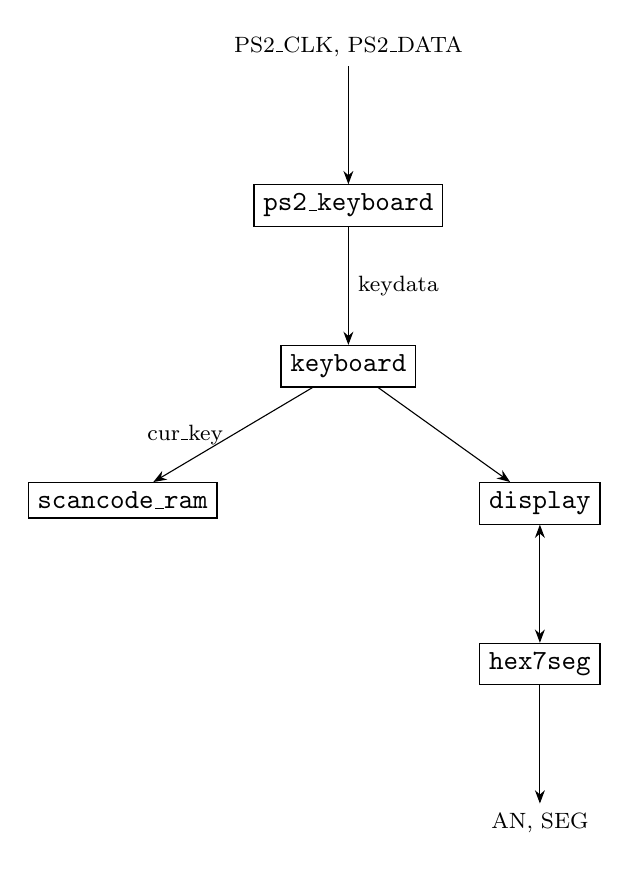
\begin{tikzpicture}[>=Stealth, node distance=1.5cm,
        every node/.style={draw}]
        \node (ps2) {\texttt{ps2\_keyboard}};
        \node[below=of ps2] (kb) {\texttt{keyboard}};
        \node[below left=1.2cm and 0.8cm of kb] (ram) {\texttt{scancode\_ram}};
        \node[below right=1.2cm and 0.8cm of kb] (disp) {\texttt{display}};
        \node[below=of disp] (hex) {\texttt{hex7seg}};

        \node[above=of ps2, draw=none, minimum width=0pt, font=\footnotesize] (in) {PS2\_CLK, PS2\_DATA};
        \node[below=of hex, draw=none, minimum width=0pt, font=\footnotesize] (out) {AN, SEG};

        \draw[->] (in) -- (ps2);
        \draw[->] (ps2) -- node[right, draw=none, minimum width=0pt, font=\footnotesize] {keydata} (kb);
        \draw[->] (kb) -- node[left, draw=none, minimum width=0pt, font=\footnotesize] {cur\_key} (ram);
        \draw[->] (kb) -- (disp);
        \draw[<->] (disp) -- (hex);
        \draw[->] (hex) -- (out);
    \end{tikzpicture}
    \caption{顶层模块连接示意图}
    \label{fig:top}
\end{figure}

\subsection{PS/2 协议接收}

\texttt{ps2\_keyboard} 模块负责底层串行数据接收。PS/2 协议每帧包含 1 位起始位、8 位数据位、1 位奇校验位和 1 位停止位，共 11 位。模块通过对 \texttt{ps2\_clk} 进行三级同步并检测下降沿来逐位采样，接收完整帧后校验并写入 8 深度 FIFO 缓冲区，供上层模块通过 \texttt{ready}/\texttt{nextdata\_n} 握手信号读取。

\subsection{键盘状态机}

\texttt{keyboard} 模块是本实验的核心，其状态机逻辑如下：

\begin{itemize}
    \item \textbf{空闲状态}：等待 FIFO 数据就绪。
    \item \textbf{收到 \texttt{0xF0}}：置 \texttt{is\_break} 标志，表示下一个扫描码为断码。
    \item \textbf{断码处理}：若该扫描码为修饰键（Shift/Ctrl/Alt），则清除对应标志；若为普通键且与 \texttt{cur\_key} 匹配，则清零当前键并允许下次按键计数。
    \item \textbf{通码处理}：若为修饰键则置位对应标志；否则若当前无键按下（\texttt{!pressed}），则记录扫描码并递增计数器。
\end{itemize}

通过 \texttt{pressed} 标志确保按住不放时只计数一次。

\subsection{扫描码到 ASCII 转换}

\texttt{scancode\_ram} 模块实现一个 $256\times 8$ 的 ROM 查找表，以扫描码为地址输出对应的 ASCII 码。查找表内容通过 \texttt{\$readmemh} 从预生成的 \texttt{ascii.txt} 文件加载。

其中，\texttt{ascii.txt} 由 \texttt{generate\_ascii.py} 生成，该文件是询问AI后得到的。

对于大写字母的支持，当 \texttt{left\_shift} 有效且 ROM 输出为小写字母（\texttt{0x61}--\texttt{0x7A}）时，将 ASCII 码减去 \texttt{0x20} 得到大写形式。

\subsection{数码管显示}

\texttt{display} 模块采用 8 位时分复用扫描方式驱动数码管。利用 17 位计数器的高 3 位选择当前数码管，配合 \texttt{en} 使能信号控制各位的亮灭。当 \texttt{cur\_key} 为零时（即按键松开），低四位数码管使能关闭，实现全灭效果。

\section{实验总结}

本实验的主要难点在于正确处理 PS/2 协议的时序和断码/通码序列。调试过程中需要注意 \texttt{nextdata\_n} 信号必须在读取数据后及时拉高，否则会重复读取同一扫描码。

修饰键的处理需要将其与普通键分开判断——修饰键不应被记录为 \texttt{cur\_key}，也不应参与按键计数，而是独立维护 toggle 状态并输出到 LED。

整体而言，本实验加深了对状态机设计方法的理解，同时熟悉了 PS/2 键盘接口的工作原理。

\section{实验感想}

这次实验算是第一次接触外部设备了吧，PS/2 键盘的接口比我想象中的要复杂一些。
不过好在课程提供了一个 PS/2 的适配接口，不需要从零开始写，这也大大减少了这次实验的难度。

总的来说我在实验过程中没有遇到什么问题，很快就做完了。第一次做这种偏向实际应用的实验，感觉还挺有意思的。

\end{document}